\begin{savequote}[8cm]
\textlatin{Neque porro quisquam est qui dolorem ipsum quia dolor sit amet, consectetur, adipisci velit...}

There is no one who loves pain itself, who seeks after it and wants to have it, simply because it is pain...
  \qauthor{--- Cicero's \textit{de Finibus Bonorum et Malorum}}
\end{savequote}

\chapter{\label{ch:1-intro}Introduction} 

\minitoc

\section{A plan}
Actually the very first thing to say will be the stuff about light i think, about diagnostic tools essentially always being about controlling the various properties of light (ie electromagnetic waves)

sections to include
start with the laser and our entrance into the multi-petawatt regime with no signs of stopping - ref 40 in alex savin thesis - it looks like that is saying huge growth in laser power check that and maybe write in thesis but don't include the figure. Also include description of CPA and OPCPA
what is a plasma
modelling plasma with PIC codes
intense lasers and absorption mechanisms?? yes for sure but dont do all just those just below ZVP
simulation units and similarity parameter
Frames of reference - lab, sim, ablating front sruface of plasma

what is the story? Based on first section by Alex after the abstract
Plasma is ubiquitous in our known universe and plasma provides us huge opportunities as a tool to improve our lives
(From chen) what we can see in the sky is a result of that stuff being in the plasma state.
Lasers can do so much now and are only getting more powerful all the time thanks to CPA and since developments (discuss)
Simulataneously our ability to understand the physics has been aided by an explosion in computing power (peter HEDP paper)
In this thesis we discuss some of the opportunities that relativistic laser plasma physics offers us with solid density targets - note that note about solids v gases at this point. 
Perhaps even before the debye length, define what we mean by the temperature of the plasma??

An unused statement about ion immobility
Assume for now that the ion-electron mass ratio is infinite, that is to say the ions are approximately immobile for the timescales under consideration, generally true for a fair few relativistic laser pulse cycles (In later sections the mobility of plasma ions will prove very important but for now this is ignored.).

\section{\label{sec:plasma_def}The definition of a plasma}
As outlined in F. Chen's definitive textbook `Introduction to Plasma Physics and Controlled Fusion' \cite{chen20116}, a plasma must fulfil three criteria, namely,

\begin{enumerate}
	\item Ionisation: a plasma must consist of both charged and neutral particles, of course this alone cannot define a plasma, any gas will contain some degree of ionisation;
	\item Quasineutrality: while locally there can be (often extreme) electromagnetic forces and charge concentrations at work, over the length scales of the plasma, such forces are screened out and the plasma bulk remains net neutral in charge;
	\item Collective behaviour: unlike in a gas where collisions dominate, the particles in a plasma generate electromagnetic fields that interact at a distance and thus a particle's motion depends not only on its immediate viscinity but on the surrounding plasma conditions, indeed often it is the so-called `collisionless' plasmas where collisions can be safely neglected that are of most interest, as is the focus of this thesis.
\end{enumerate}

\subsection{\label{sec:debye_length}The Debye length}
The Debye length describes the extent to which a plasma can shield electromagnetic fields within and so remain quasineutral. Consider an infinitely extending plasma with a test charge placed at some point, then what would be the potential $\phi(\mathbf{x})$? If the plasma had no kinetic energy, the charged particles would arrange themself immediately ajacent to the test charge and once this equilibrium state was reached there would be no electromagnetic fields present. Realistically the plasma will have some temperature, likely a very large temperature and so some particles will be able to escape the potential of the test charge and thus leak electromagnetic fields into the plasma bulk. Poisson's equation reads
\begin{equation}\label{eq:poisson}
	\epsilon_0\nabla^2\phi = -e(Zn_i - n_e),
\end{equation}
where $\epsilon_0 = \qty{8.854e-12}{F.m^{-1}}$ is the permittivity of free space, $e = \qty{1.602e-19}{C}$ is the charge of an electron, $Z$ is the plasma ion charge in units of $e$ and $n_i$ and $n_e$ are the number densities of plasma ions and electrons.

Since the electrons are significantly more mobile than the ions due to their lower mass, it is in general the electrons and not the ions that respond to the test charge and the ions can be assumed to provide a constant background of positive charge density.
If the number density of electrons follows a Boltzmann temperature distribution in the presence of a potential energy $-e\phi$, then
\begin{equation}\label{eq:nj_boltzmann}
	n_e= n_{e,0}e^{e\phi/KT_e},
\end{equation}
where $n_{e,0}$ is the electron number density far from the test charge, $n_i = n_{e,0}/Z$ and $KT_e$ is the electron temperature. Note that in plasmas it is very common for different species to have differing temperatures depending on the mechanism for energy absorption and the timescales for collisions compared to the timescale of the study.

Substituting equation \ref{eq:nj_boltzmann} into equation \ref{eq:poisson} and Taylor expanding the exponential term in the limit that the plasma is weakly coupled ($e\phi << KT_e$), obtains 
\begin{equation}\label{eq:poisson_debye2}
	\nabla^2\phi = \frac{\phi}{\lambda_D^2},
\end{equation}
where
\begin{equation}\label{eq:debye}
	\lambda_D \equiv \sqrt{\frac{\epsilon_0KT_e}{n_ee^2}},
\end{equation}
is the \textit{Debye length} and describes the thickness of the charge sheath surrounding the test charge. For quasineutrality to hold for the plasma bulk, its spatial dimensions must extend beyond a few Debye lengths.

\subsection{\label{sec:plasma_parameter}The plasma parameter}
In order for the above description to be statistically valid, there must be a large number of charged particles within the shielding sheath. The number of particles within the \text{Debye sphere} can be computed as
\begin{equation}\label{eq:plasma_parameter}
	N_D = \frac{4}{3}\pi\lambda_D^3n.
\end{equation}
Note that, as discussed above, in most cases it is most suitable to choose the number density $n$ to be the number density of electrons. To ensure the plasma is suitably ionised (criterion 1) and that the plasma engages in collective behaviour (criterion 3),
\begin{equation}\label{eq:plasma_parameter_condition}
	N_D >>> 1.
\end{equation}
\subsection{\label{sec:plasma_frequency}Collisionality and the plasma frequency}
Collective behaviour not only depends on the ability for large numbers of particles to interact via electromagnetic forces but that these forces dominate over collisions in describing particle trajectories. Taking $\omega$ as the typical frequency of plasma oscillations and $\tau$ as the average time between collisions, for a plasma (as opposed to a gas) must satisfy
\begin{equation}\label{eq:plasma_frequency_condition}
	\omega\tau > 1.
\end{equation}
It now remains to determine what is the typical frequency of collisions in a given plasma. While the types of plasma waves and their associated frequencies of oscillation are multitudinous, the characteristic frequency, the \textit{plasma frequency}, $\omega_p$, is the most straightforward. It describes the response of electrons to charge imbalances within an infinite uniform plasma at rest in the absence of magnetic fields or temperature fluctuations. As noted in section \ref{sec:debye_length}, the ions provide a constant backgorund of positive charge.

Consider an semi-infinite plasma existing for $x>0$, with electron density $n_e$ and ion density $n_e/Z$ of charge state $Z$\footnote{This description has direct relevance to the Zero Vector Potential mechanism which will be made clear later.}. Suppose the electron fluid is displaced by some perfectly isotropic force into the plasma bulk a distance $(\Delta x) \hat{\mathbf{x}}$ as in figure \ref{fig:introplasmafrequency}. 
\begin{figure}
	\centering
	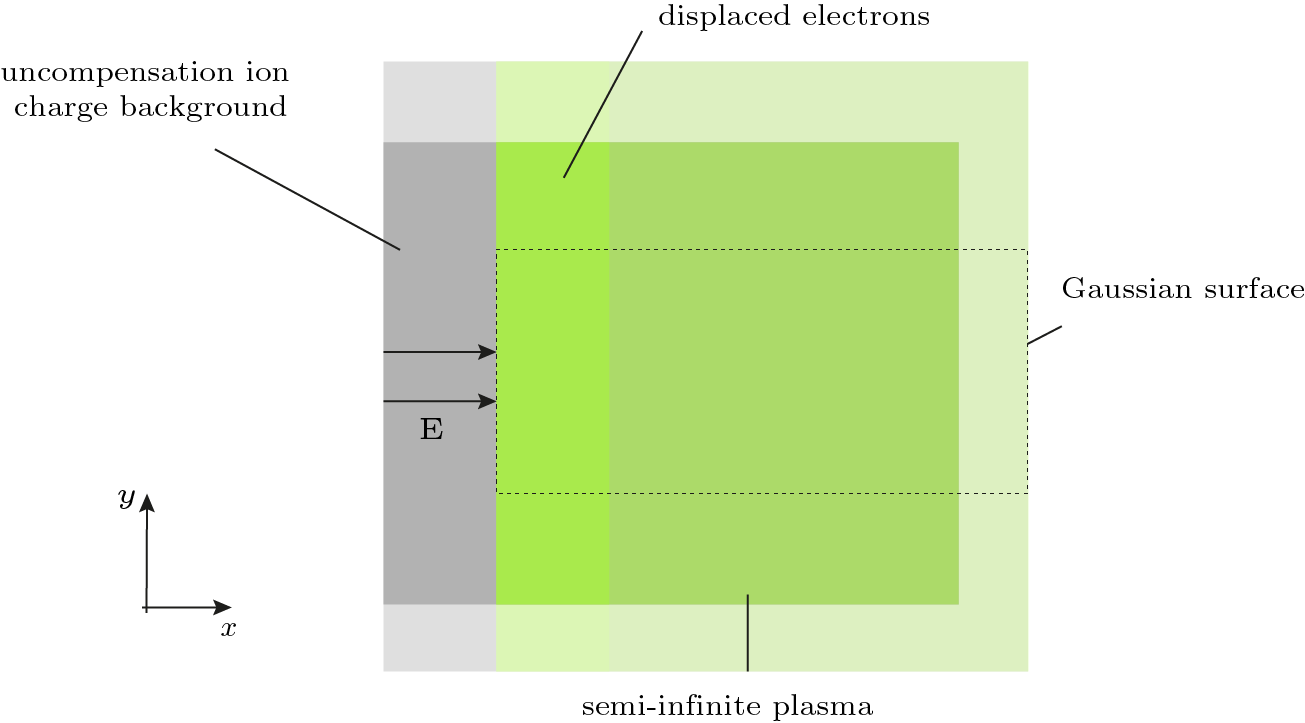
\includegraphics[width=0.7\linewidth]{figures/intro/intro_plasma_frequency}
	\caption{Diagram to illustrate the plasma frequency derivation.THIS FIGURE NEEDS E POINTING THE OTHER WAY}
	\label{fig:introplasmafrequency}
\end{figure}
The total charge of displaced electrons within a surface area of $\sigma$ is 
\begin{equation}\label{eq:intro_Q}
	Q = -en_\mathrm{e}\sigma\Delta x.
\end{equation}
Applying Gauss' law to the surface detailed in figure \ref{fig:introplasmafrequency}, the uncompensated charge leads to 
\begin{equation}\label{eq:intro_E}
	-\sigma E\hat{\mathbf{x}}= \frac{Q}{\epsilon_0}\hat{\mathbf{x}} = -\frac{en_e\sigma\Delta x}{\epsilon_0}\hat{\mathbf{x}}
\end{equation}
at the electron surface. By the Lorentz force, the displaced electrons will experience a restoring force, $-eE\hat{\mathbf{x}}$, perpendicular to the surface due to the electron-ion charge imbalance. The equation of motion for electrons on that surface is therefore
\begin{equation}\label{eq:intro_sho}
	m_e\frac{\mathrm{d}^2\Delta x}{\mathrm{d}t^2} = -eE = -\frac{e^2n_e}{\epsilon_0}\Delta x.
\end{equation}
Equation \ref{eq:intro_sho} clearly describes a simple harmonic oscillator with a characteristic frequency given by the plasma frequency,
\begin{equation}
	\omega_p = \sqrt{\frac{e^2n_e}{m_e \epsilon_0}}.
\end{equation}



\section{The Lawson-Woodward theorem}\label{sec:intro-lawson_woodward}
The Lawson-Woodward theorem states that there can be no net electron energy gain using laser fields \cite{esarey_2009_PhysicsLaserdrivenPlasmabaseda}, quite at odds with one of the primary aims of this thesis, that is, the acceleration of electrons. There are, however, several conditions that must be met, namely,
\begin{enumerate}
	\item The interaction region is infinite;
	\item The interaction  occurs in a vacuum;
	\item The electron is ultra-relativistic ($v\approx c$) along the acceleration gradient;
	\item No electro- or magnetostatic fields are present;
	\item Non-linear effects are neglected.
\end{enumerate}
Several of these will be applicable to the various accelerations of electrons considered. It is this final condition that is most damning, throughout this thesis the ultra-relativistic laser pulses under consideration ensure non-linear effects cannot be neglected. It is indeed such non-linearities that are of interest.

\section{Relativistic effects}
The descriptor `Relativistic' is applied liberally in this thesis. When applied to electromagnetic fields or laser pulses it refers to 
\begin{equation}
	a_0 \gg 1.
\end{equation}
When applied to particles, their speeds are
\begin{equation}
	v \approx c.
\end{equation}
A relativistic laser pulse will accelerate electrons to relativistic velocities in a fraciton of a laser pulse cycle. Consider an electron in the presence of a uniform electric field of magnitude $a_0 = 100$, an intensity accessible by current state of the art laser facilities. The work done on that particle by the field is 
\begin{equation}
	U = (\gamma -1)m_\mathrm{e}c^2 = \int \mathbf{E}\cdot \mathrm{d} \mathbf{x},
\end{equation}
where 
\begin{equation}
	\gamma = \frac{1}{\sqrt{1-\beta^2}}.
\end{equation}
The field will accelerate an electron to a $\beta = 0.99$, corresponding to $\gamma \approx 7$, in less than 1 \% of a corresponding laser pulse wavelength.

\subsection{Conservation of generalised transverse momentum}\label{sec:intro_conservation-generalised-mometum}
Consider a holonomic system of $N$ relativistic particles under the influence of electromagnetic forces. A particle $j$ with charge $e_j$ and mass $m_\mathrm{j}$ experiences a scalar potential,
\begin{equation}
	U_{j} = e_j(\Phi - \mathbf{A} \cdot \mathbf{v}_{j})
\end{equation}
and hence the system is described by the Lagrangian
\begin{equation}
	L = \sum^N_{j=1}\left( - m_\mathrm{j}c^2\sqrt{1-\beta^2_\mathrm{j}} - e_j(\Phi - \mathbf{A} \cdot \mathbf{v}_\mathrm{j}) \right),
\end{equation}
where $\beta^2_j = \mathbf{v}_\mathrm{j}\cdot\mathbf{v}_\mathrm{j} /c^2$ and $\mathbf{v}_j = \mathrm{d}\mathbf{x}_j/\mathrm{d}t$ \cite{goldsteinClassicalMechanics2013}.
The generalised momentum corresponding to coordinate $x_j$ is
\begin{equation}
	p_{j,x} = \frac{\partial L}{\partial \dot{x}_j} = m_j\dot{x}_j + e_jA_x,
\end{equation}
thus, the generalised momentum describes both the linear mechanical momentum and the momentum of the electromagnetic field. Via Noether's theorem, if $L$ is independent of $x_j$, \textit{i.e.} spatially homogeneous along $x$ for particle $j$, then 
\begin{equation}\label{eq:intro-transverse_momentum_differential_equation}
	\dot{p}_{j,x} = 0
\end{equation}
since
\begin{equation}
	\frac{\mathrm{d}}{\mathrm{d}t}\left(\frac{\partial L}{\partial \dot{x}_j}\right) = \frac{\partial L}{\partial x_j}.
\end{equation}

Consider a linearly polarised Gaussian laser pulse, with axis of polarisation along $x$ incident on a solid target at rest. Then $A_x$ is approximately constant along $x$ near the beam centre\footcite{Constant relative to the scale of typical electron trajectories in such an interaction.}. Integrating equation \ref{eq:intro-transverse_momentum_conservation_no_initial_momentum} and noting that initially there is no linear or electromagnetic momentum at the target, the generalised transverse momentum conservation equation for an electron in the laser field is
\begin{equation}\label{eq:intro-transverse_momentum_conservation_no_initial_momentum}
	p_\mathrm{T} = eA,
\end{equation}
where $p_\mathrm{T}$ is the electron momentum along the polarisation axis of the laser pulse and $A$ it the laser pulse vector potential.

Note that this is only valid provided the electron does not radiate along the direction of polarisation as discussed by Sokolov \textit{et al} \cite{sokolovDynamicsEmittingElectrons2009}. The implications of `Radiation Reaction' are discussed in the following section.

\section{QED effects}
We are now at the cusp of \ac{SF-QED} laser-plasma physics. Access to this regime will enable the testing of decades old theoretical predictions. Already Fedeli \textit{et al} have shown in simulations that current PW-class laser facilities can access the regime using an all-optical set up based on laser-solid surface interactions \cite{fedeli_2020_ProbingStrongfieldQED}. The primary two SF-QED phenomena to be accessed are Radiation Reaction and multi-photon Breit-Wheeler electron pair production. Brief introductions to these phenomena are now presented.


\subsection{High-energy photon emission and radiation reaction}
When a charged particle undergoes an acceleration, it emits electromagnetic radiation. If the electromagnetic field is sufficiently strong, \textit{i.e.} approaching the Schwinger Limit in the rest frame of the particle, then a non-neglible fraction of particle momentum can be transferred to the emitted high energy photon via inverse Compton scattering, substantially impacting the dynamics of the accelerated particle. This back reaction is known as Radiation Reaction.



Note for in simulation section: 'The processes discussed in this section bring into play a characteristic length [the classical radius of the electron 

in classical electrodynamics (CED) or the standard Compton wavelength 

in quantum electrodynamics (QED)]. As a result, a simulation will require the user to define the absolute scale of the system by defining the referencangularfrequencySI parameter' '
Also there are a list of assumptions in smilei that I should state in the simulation section and demonstrate they are all fine.

\subsection{Multi-photon Breit-Wheeler pair production}

(This has been written up from smilei but should probs get reference elsewhere??) > check out savin thesis

Multi-photon Breit-Wheeler pair production, also known as non-linear Breit-Wheeler is the decay of a high energy photon, typically produced via \ac{RR}, into an electron-positron pair in the presence of a strong electromagnetic field, explicitely,
\begin{equation}
	\gamma + n\omega \to e^- + e^+.
\end{equation}
The strength of the effect is dependent on the lorentz invariant photon quantum parameter,
\begin{equation}
	\chi_\gamma = \frac{\gamma_\gamma}{E_\mathrm{s}} \sqrt{(\mathbf{E}_\perp + \mathbf{c}\times \mathbf{B}^2},
\end{equation}
where $E_\mathrm{s} = \qty{1.3e18}{V.m^{-1}}$ is the Schwinger electric field, $\gamma_\gamma = \epsilon_\gamma /m_\mathrm{e}c^2$, the normalised photon energy and $\mathbf{E}_\perp$ the electric field perpendicular to the photon propagation direction. Cite Smilei and say, in a constant E-field, the rate of pair production increases rapidly up to $\chi_\gamma \approx 10$ at which point it saturates and slowly reduces.


If the electron radiates all its energy to the photon, for the ZVP mechanism, at the point of emission one finds,
\begin{equation}
	\chi_\gamma = |\mathbf{E}|\frac{1 + \frac{a^2_0}{\bar{n}_\mathrm{e}}}{E_\mathrm{s}} \sqrt{2},
\end{equation}
The chi parameter will change rapidly once the transition to QED ZVP has occured due to the change in scaling.


\section{Simulations}
\subsection{Particle-In-Cell codes}

I think put this in the main intro section. Then start PIC codes with discretisation of the Vlasov-Maxwell system of equations.

\subsubsection{The Vlasov-Maxwell system of equations}
A collisionless and fully ionised plasma, as relevant to this thesis, is fully described in the kinetic description by the Vlasov-Maxwell system of equations \cite{derouillatSmileiCollaborativeOpensource2018}. Each plasma species, $s$, of particles with mass $m_s$ and charge $q_s$ is described by its distribution function $f_s(t,\mathbf{x},\mathbf{p})$ at time $t$, position $\mathbf{x}$ and momentum $\mathbf{p}$. The distribution satisfies the Vlasov equation, that is,
\begin{equation}
	(\partial_t + \frac{\mathbf{p}}{m_s\gamma} \cdot \nabla + \mathbf{F}_\mathrm{L} \cdot \nabla_\mathbf{p})f_s = 0,
\end{equation}
where $\gamma = \sqrt{1+\mathbf{p}^2/(m_sc)^2}$ is the relativistic Lorentz or gamma factor of the distribution and 
\begin{equation}
	\mathbf{F}_\mathrm{L} = q_s(\mathbf{E} + \mathbf{v} \times \mathbf{B})
\end{equation}
is the Lorentz force that acts on a particle with velocity $\mathbf{v}  = \mathbf{p}/m_s\gamma$. The electric $\mathbf{E}(t,\mathbf{x})$ and magnetic $\mathbf{B}(t,\mathbf{x})$ fields that create the force must satisfy Maxwell's equations,
\begin{equation}
	\nabla \cdot \mathbf{B} = 0,
\end{equation}
\begin{equation}
	\nabla \cdot \mathbf{E} = \frac{\rho}{\epsilon_0},
\end{equation}
\begin{equation}
	\nabla \times \mathbf{B} = \mu_0 \mathbf{J} + \mu_0 \epsilon_0 \partial_t \mathbf{E},
\end{equation}
\begin{equation}
	\nabla \times \mathbf{E} =-\partial_t \mathbf{B}.
\end{equation}
Here $\epsilon_0$ and $\mu_0$ are the vacuum permittivity and permeability respectively.

This self-consistent system of equations describes the dynamics of plasma particles within electromagnetic fields. The particles then modify the fields via their charge and current densities,
\begin{equation}
	\rho(t,\mathbf{x}) = \sum_s q_s \int d^3pf_s(t,\mathbf{x},\mathbf{p}),
\end{equation}
and 
\begin{equation}
	\mathbf{J}(t,\mathbf{x}) = \sum_s q_s \int d^3p\mathbf{v}f_s(t,\mathbf{x},\mathbf{p}),
\end{equation}
respectively.

\subsubsection{Discretisation of the Vlasov-Maxwell equations}
Finding numerical solutions to the Vlasov-Maxwell equations is no straightforward task, there are codes that are capable such as Valis \textbf{**CITE**}, however, the requirement for very high resolution in both position and momentum is exceedingly costly and use of such codes are limited in their size, duration and spatial dimensions. A more tractable approach is to discretise the distribution function into $N_s$ `quasi-particles'\footnote{Originally introduced by Langdon and Birdsall as `clouds' \cite{langdonTheoryPlasmaSimulation1970}.}  (often referred to as `macro-particles' in practice as they typically represent a large number of real particles), such that
\begin{equation}
	f_s(t,\mathbf{x},\mathbf{p}) = \sum^{N_s}_{p=1} w_p S(\mathbf{x}-\mathbf{x}_p(t))\delta (\mathbf{p}-\mathbf{p}_p(t)),
\end{equation}
where $w_p$ is the quasi-particle's weight, $\mathbf{x}_p$ and $\mathbf{p}_p$ are its position and momentum respectively, $\delta$ is the Dirac-delta distribution and $S(\mathbf{x})$ the shape-function chosen to represent the quasi-particle. The Vlasov equation is then integrated along the continuous trajectories of the quasi-particles while Maxwell's equations are solved on a discrete spatial grid of `cells'. Such a code is aptly named a `\ac{PIC}' code.

% TODO: \usepackage{graphicx} required
\begin{figure}
	\centering
	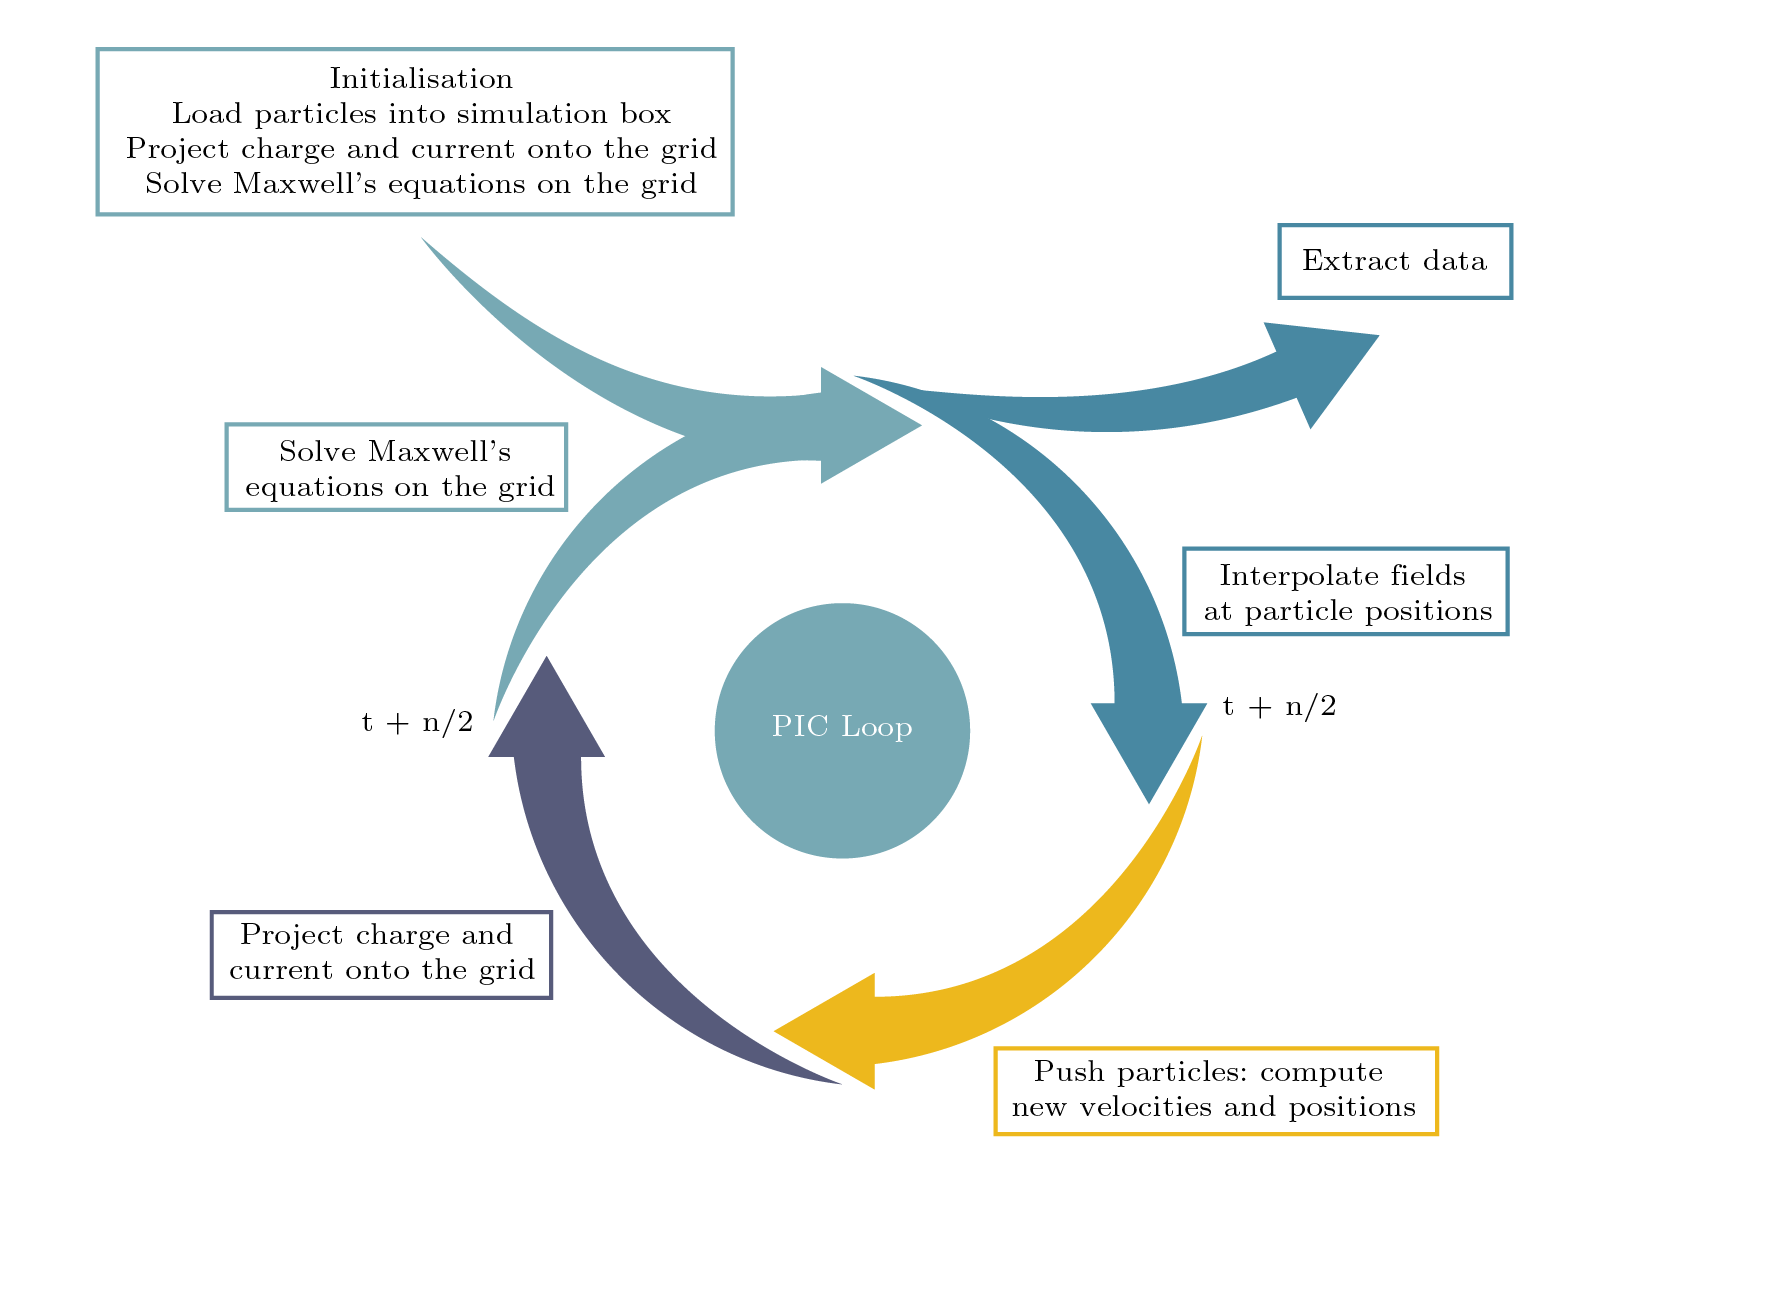
\includegraphics[width=\linewidth]{figures/intro/intro_PIC_cycle-01}
	\caption[Diagram of the PIC code algorithm]{Diagram of the PIC code algorithm}
	\label{fig:intropiccycle-01}
\end{figure}


\subsubsection{Smilei}
Smilei (for Simulating Matter Irradiated by Light at Extreme Intensities) is a modern collaborative, massively-parallel, fully relativistic and open source plasma physics PIC code and was the main workhorse for this thesis\footnote{At points benchmarks agaist the EPOCH and Osiris PIC codes were performed.}. Produced by M. Grech's team(CHECK THIS) at École Polytechnique \cite{derouillatSmileiCollaborativeOpensource2018}, its development was motivated by the rapid development of multi-petawatt facilities globally including their local Apollon laser and by supercomputing power which has `skyrocketed' in recent years \cite{derouillatSmileiCollaborativeOpensource2018}. Indeed, the work in this thesis with 3D simulations required over \qty{1e6}{cores}.


\subsubsection{Reference quantities}
This needs rewording so as not to be the same as paper.

%With the vast range of magnitudes associated with multi-petawatt and femtosecond laser pulses, solid density plasmas, micrometre wavelengths and attosecond bunches, it is much more efficient to convert to dimensionless normalised quantities. The standard four that describe the dynamics of the system \cite{BOUCHARD THESIS??} correspond directly to each of these. The three asso- ciated with the laser are: the temporal parameter, ωLτ, where τ is the pulse duration, the spatial parameter, λL/R, where λL is the wavelength and R the beam width, and the intensity parameter, the normalised vector po- tential, a0 = eEL/(mecωL), where EL is the peak laser electric field strength, and e and me are the charge and mass of an electron.
%For the plasma, the key parameter is the density rel- ative to the critical density, n ̄e = ne/nc, here ne is the electron density and nc = ε0 me ωL2 /e2 is the critical den- sity at which the plasma becomes opaque to the laser electric field, assuming relativistic effects can be ignored.
%Relativistic similarity theory states that the laser- plasma interaction does not depend on n ̄e and a0 inde- pendently but via the relativistic similarity parameter
%S=n ̄e, (1) a0
%essentially accounting for relativistic effects in the over- density of the plasma. Previous work on the ZVP mech- anism has suggested that the ZVP regime is valid for relativistic interactions, a0 > 1, with S ≥ 1. For S < 1, the onset of relativistically self-induced transparency ef- fects [42] renders the model invalid. Equally, for large a0, the onset of QED effects should cause breakdown of rel- ativistic similarity. Here the validity of the ZVP model is tested across this parameter space for the first time.

\subsubsection{Reference units}
To great convenience, Smilei operates in normalised units. This normalisation is not chosen \textit{a priori}, instead results can be scaled by an arbitrary reference angular frequency. This is extremely useful when working with boosted frames of reference. As this thesis focuses on the interaction of a laser pulse with plasma, the laser pulse angular frequency, $\omega_\mathrm{L}$ is set as the frequency of reference. A list of the most common normalisations are given in table \ref{tab:intro-normalisations}.

\begin{table}
\begin{center}
\begin{tabular}{ccc}
	 \hline \hline
	Units of & SI units & Normalisation \\
	\hline
	velocity & \unit{m.s^{-1}} & $c$ \\
	charge & C & $e$ \\
	mass & kg & $m_\mathrm{e}$ \\
	momentum & \unit{kg.m.s^{-1}} & $m_\mathrm{e}c$ \\
	energy/temperature & J & $m_\mathrm{e}c^2$ \\
	time & s & $\omega^{-1}_\mathrm{L}$ \\
	length & m & $c/\omega_\mathrm{L}$ \\
	number density & \unit{m^{-3}} & $n_\mathrm{c}$ \\
	electric field & \unit{V.m^{-1}} & $m_\mathrm{e}c\omega_\mathrm{L}/e$ \\
	\hline \hline
\end{tabular}
	\caption{\label{tab:intro-normalisations} Smilei normalisations for common quantities with the laser angular frequency $\omega_\mathrm{L}$ set at the reference angular frequency.}
\end{center}
\end{table}




